\chapter{Grundlagen}



% Wortherkunft ====================================
\section{Wortherkunft}
\label{sec:wortherkunft}

\begin{description}
\item[Bus] „omnibus“ lat. „für alle“
\item[hier:] Kommunikationsmedium „für alle“
\item[klass. „shared medium“:] Was einer der Teilnehmer auf dem Medium sendet, hören (potentiell) alle Teilnehmer gleichzeitig mit.
\end{description}
% =================================================



% Topologien ======================================
\section{Topologien von „Computernetzen“}
\label{sec:topologien}

\subsubsection{Stern}
\begin{figure}[htbp]
  \centering
  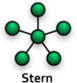
\includegraphics[scale=0.7]{Stern-Topologie.png}
  \caption{Stern-Topologie}
\end{figure}
Es gibt einen zentralen „Sternverteiler“ in der Mitte und dedizierte Leitungen von diesem zu jedem der Teilnehmer. Üblicherweise ist der Sternverteiler \underline{nicht} auch ein „normaler Teilnehmer“.\\

\subsubsection{Ring}
\begin{figure}[htbp]
  \centering
  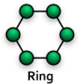
\includegraphics[scale=0.7]{Ring-Topologie.png}
  \caption{Ring-Topologie}
\end{figure}
Jeder Teilnehmer hat genau einen Vorgänger und einen Nachfolger, mit denen er jeweils verbunden ist.

\subsubsection{Bus}
\begin{figure}[htbp]
  \centering
  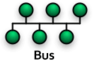
\includegraphics[scale=0.7]{Bus-Topologie.png}
  \caption{Bus-Topologie}
\end{figure}
Es gibt lediglich eine „Leitung“ als „shared medium“, mit welchem jeder Teilnehmer über eine „Stichleitung“ verbunden ist.

\subsubsection{Maschennetz}
\begin{figure}[htbp]
  \centering
  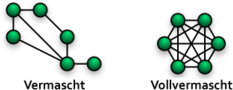
\includegraphics[scale=0.7]{Vermascht-Topologie.png}
  \caption{Maschen-Topologie}
\end{figure}
Jeder Teilnehmer hat zu beliebig vielen anderen Teilnehmern jeweils eine dedizierte Verbindung. Beim Spezialfall Vollvermascht hat jeder Teilnhemer eine Verbindung zu demem anderen Teilnehmer.

\subsubsection{Baum}
\begin{figure}[htbp]
  \centering
  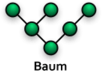
\includegraphics[scale=0.7]{Baum-Topologie.png}
  \caption{Baum-Topologie}
\end{figure}
Die Baumtopologie ist eine hierarchische Topologie. Ausgehend von einem „Wurzel Teilnehmer“ gibt es jeweils ein oder mehrere Verbindungen zu Teilnehmern der nächsten Hierarchieebene.

\subsubsection{Linie}
\begin{figure}[htbp]
  \centering
  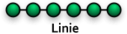
\includegraphics[scale=0.7]{Linie-Topologie.png}
  \caption{Linien-Topologie}
\end{figure}
Jeder Teilnehmer ist mit maximal zwei Teilnehmern verbunden. Es gibt einen Anfang und ein Ende.
% =================================================



% Bustopologie ====================================
\section{Verwenden alle „Bussysteme“ eine Bustopologie?}
\begin{table}[h]
\centering
\begin{tabular}{c|c}
\textbf{Bustopologie} & \textbf{Bustopologie} \\ 
\hline 
Ethernet in BNC-Verkabelung & USB: Baum \\ 
\hline 
ProfiBus & MOST: Ring \\ 
\hline 
WLAN & Ethernet in TP-Verkabelung: Baum \\ 
\hline
IDE (P-Data) & (S-ATA)\\
\hline
PCI & (PCI-Express)\\
\hline
SCSI & (SAS (Seriell Attached SCSI))\\
\hline
 & Firewire: vermaschtes Netz\\
 & mit Einschränkungen
\end{tabular}
\caption{Einordnung von Technologien in Bussysteme}
\label{tab:bussystem_or_not}
\end{table} 
Viele der heutigen „Bussysteme“ sind physikalisch keine \underline{Busse}, sondern nur noch logisch/protokolltechnisch auf einer höheren Ebene.
% =================================================



% Spezielle Aufgaben von Bussystemen ==============
\section{Spezielle Aufgaben von Bussystemen}
\label{sec:spezielle_Aufgaben_Bussysteme}
Speziell bei Bussystemen zu lösende Aufgaben:
\begin{itemize}
\item Medienzugriff
\item Adressierung
\end{itemize}
% =================================================

\section{Entwicklung eines Medienzugriffsverfahrens am Bsp. CSMA/CD}
\begin{description}
\item[ALOHA] (erstes Bussystem für die Entwicklung des CSMA/CD): Bei Bedarf wird gesendet.
\par
Problem: Zwei oder mehr Sender können gleichzeitig senden, dadurch werden alle Sendungen gestört und müssen verworfen werden.
\par
Aufgrund der nicht zu hohen Anzahl an Teilnehmern und der geringen Datenmenge ist die Kollisionswahrscheinlichkeit gering und das Verfahren funktioniert trotzdem (Kollision muss auf höherer Protokollebene durch zweiten Sendeversuch erkannt und behoben werden).

\item[Slotted ALOHA] (Weiterentwicklung des ALOHA): Die Verfügbarkeit des Mediums wird in Zeitschlitze eingeteilt (synchron für alle Teilnehmer), dabei umfasst jede Sendung genau einen Zeitschlitz.
\begin{itemize}
\item[$\Rightarrow$] verringerte Kollisionswahrscheinlichkeit, da Kollisionen nur zu Beginn des Zeitschlitzes und nicht mehr in dessen Verlauf stattfinden können \item[$\Rightarrow$] nur genau dieser Zeitschlitz ist von der jeweiligen Kollision betroffen.
\end{itemize}

\item[CSMA] (Carrier Sense Multiple Access): Vor dem Beginn der Übertragung wird der Übertragungskanal abgehört, ob bereits eine Sendung stattfindet.\\
Falls Ja $\Rightarrow$ späterer Versuch\\
Falls Nein $\Rightarrow$ Sendeversuch möglich
\par
\textbf{Achtung:} CSMA ist nur als Weiterentwicklung von “Unslotted” ALOHA möglich
Bei Slotted ALOHA ist der Übertragungskanal unmittelbar zu Beginn des Zeitschlitzes immer frei!
$\Rightarrow$ CSMA bringt in diesem Fall \underline{keinen Vorteil!}
\par
Jetzt: Kollisionen können nur “quasi-gleichzeitig” stattfinden, d.h. innerhalb eines Zeitfensters, welches der Signalverzögerung zwischen den beiden an der Kollision beteiligten Stationen entspricht.
\par
Vorher bei Slotted ALOHA: Kollision immer dann, wenn während des gesamten vorherigen Zeitschlitzes bei zwei oder mehreren Stationen ein Übertragungswunsch entstanden ist.\\
$\Rightarrow$ CSMA reduziert die Kollisionswahrscheinlichkeit, sofern die Übertragungsverzögerung kürzer als ein Zeitschlitz bei Slotted ALOHA ist.

\item[CSMA/CD] (CSMA with Collision Detection): Kollisionserkennung, man hört den Übertragungs-kanal auch während der eigenen Übertragung ab und vergleicht das gesendete mit dem empfangenen Signal. Ungleichheit bedeutet Kollision.\\
Sender, welcher die Kollision erkennt bricht die Übertragung ab und sendet stattdessen ein sog. JAM Signal, welches den anderen Stationen (insbesondere den Empfängern) signalisiert, dass eine Kollision stattgefunden hat und die bisherige Sendung verworfen werden muss.
\begin{itemize}
\item[$\Rightarrow$] keine Verringerung der Kollisionswahrscheinlichkeit 
\item[$\Rightarrow$] Verkürzung der Zeitdauer in der der Übertragungskanal mit Störung (und damit nutzlos) belegt ist, weil direkt abgebrochen wird
\end{itemize}
    
\begin{figure}[htbp]
  \centering
  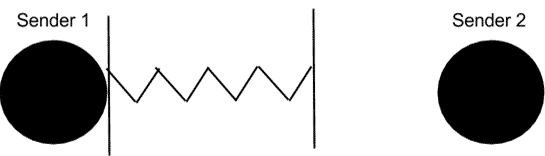
\includegraphics[width=10cm]{CSMA_CD.png}
  \caption{Kollisionserkennung CSMA/CD}
\end{figure}

Zur sicheren Kollisionserkennung muss die Mindestlänge eines Paketes auch und gerade beim 1. Sender die doppelte Signalverzögerung aufweisen $\Rightarrow$ ansonsten bekommt der 1. Sender das JAM Signal des zweiten Senders erst nach dem Ende seiner eigenen Übertragung mit $\Rightarrow$ zu spät.

\item[Zahlenwert] (“klassisches CSMA/CD”):
\begin{itemize}
\item Übertragungsverzögerung: $12,5\mu s$
\item max. Ausdehnung: $\approx2500m$
\item Übertragungsrate: $10MBit/s$
\item Geschwindigkeit in einem Kupferkabel: $200 000 km/s$
\begin{itemize}
\item[]$v=st \Rightarrow t=sv$
\item[]$v\approx\frac{2}{3}c\approx2*10^{8}\frac{m}{s}$
\item[]$t=\frac{2500m}{200*10^{6}\frac{m}{s}}=12,5s$
\item[]$r=\frac{m}{t} m:Speichermenge (in bit)$
\item[]$m=r*t=125bit \approx 16Byte$
\end{itemize}
\item in der Realität 42 oder 46 Byte

\item Folgerung für Fast Ethernet (100Mbit/s):
\begin{itemize}
\item[]keine größere minimale Datenmenge!
\item[]sondern kleinere “Kollisionsdomänen”
\item[]mehrere Kollisionsdomänen müssen über Switches (“Store and Forward”) und nicht einfach Hubs (Signalverstärker) verbunden werden!
\end{itemize}

\item Folgerung für Gigabit Ethernet (1GBit/s):
\begin{itemize}
\item[]für jede Übertragungsrichtung zwischen jeweils zwei Geräten (Endgerät oder Switch -  kein HUB erlaubt) gibt es einen eigenen Übertragungskanal $\Rightarrow$ Vollduplex $\Rightarrow$ keine Kollisionen möglich!
\end{itemize}
\end{itemize}

\end{description}